\documentclass[tikz,border=4pt]{standalone}
\usepackage[T1]{fontenc}
\usepackage[utf8]{inputenc}
\usepackage{amsmath,amssymb}
\usepackage{helvet}
\renewcommand{\familydefault}{\sfdefault}
\usepackage{pgfplots}
\pgfplotsset{compat=1.17}
\usetikzlibrary{arrows.meta,positioning,calc,fit,backgrounds,shapes.geometric}

\definecolor{cVis}{HTML}{1F77B4}
\definecolor{cTxt}{HTML}{D62728}
\definecolor{cProj}{HTML}{2CA02C}
\definecolor{cLLM}{HTML}{9467BD}
\definecolor{cConv}{HTML}{FF7F0E}
\definecolor{cAtt}{HTML}{17BECF}
\definecolor{cGray}{HTML}{7F7F7F}

\tikzset{
  blk/.style={draw, rounded corners=2pt, minimum height=8mm, align=center, font=\footnotesize, thick},
  tok/.style={draw, minimum size=3.2mm, inner sep=0pt},
  arr/.style={-{Stealth[length=2mm]}, thick},
}

\begin{document}
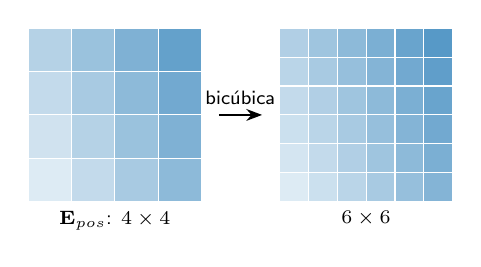
\begin{tikzpicture}[scale=.55]
  \foreach \i in {0,...,3}{\foreach \j in {0,...,3}{\pgfmathsetmacro{\c}{15+12*\i+6*\j}\fill[cVis!\c] (\i,\j) rectangle ++(1,1);\draw[white] (\i,\j) rectangle ++(1,1);}}
  \node[below,font=\scriptsize] at (2,0) {$\mathbf{E}_{pos}$: $4\times4$};
  \draw[arr] (4.4,2) -- (5.4,2) node[midway,above,font=\scriptsize]{bicúbica};
  \foreach \i in {0,...,5}{\foreach \j in {0,...,5}{\pgfmathsetmacro{\c}{15+8*\i+4*\j}\fill[cVis!\c] (5.8+\i*0.667,\j*0.667) rectangle ++(0.667,0.667);\draw[white] (5.8+\i*0.667,\j*0.667) rectangle ++(0.667,0.667);}}
  \node[below,font=\scriptsize] at (7.8,0) {$6\times6$};
\end{tikzpicture}
\end{document}
